\chapter{Copyright-Protected Language Generation via Adaptive Model Fusion}
\label{chap:cpfuse}
\chaptermark{CP-Fuse for Copyright-Protected Generation}

This chapter studies copyright protection for language generation. Large language models have achieved undeniable success, but they also risk reproducing copyrighted material from their training data. To address this problem, the chapter introduces Copyright-Protecting Model Fusion (CP-Fuse), an inference-time strategy that combines models trained on disjoint sets of copyrighted material to prevent regurgitation. CP-Fuse substantially reduces copyright-infringement metrics across text and code generation tasks, preserves utility, and can be combined with other protective measures.

This chapter is based on joint work with Konstantin Donhauser, Francesco Pinto, and Fanny Yang. The work was led by the author of this thesis, and appeared as \citet{abad2025copyright}.

\section{Motivation and Scope}

Large Language Models (LLMs), such as GPT-4 \citep{achiam2023gpt} and Gemini \citep{team2023gemini}, have achieved undeniable success. However, they also present a significant challenge: the risk of reproducing copyrighted material from their training data \citep{sag66new,yu2023codeiipprompt,karamolegkou2023copyright}. With the widespread adoption of these models for generating new text and code, the risk of large-scale copyright violations has become a pressing issue, as highlighted by several multi-million dollar lawsuits \citep{henderson2023foundation}. Consequently, preventing copyright infringement in language models has become a critical focus for researchers and practitioners alike.

The \emph{fair use} doctrine (17 U.S.C. 107) provides a framework to mitigate liability for copyright infringement, spurring interest in techniques that allow models to use protected works in transformative ways that do not harm their market value \citep{henderson2023foundation}. Since verbatim reproduction of copyrighted material often arises from the memorization of training data \citep{carlini2021extracting,Somepalli2022DiffusionAO,carlini2023quantifying,mm_mem2024}, a natural goal is to reduce memorization without destroying the usefulness of the model. The literature has therefore explored interventions at several stages of the model pipeline, from data curation and training-time regularization to inference-time protection. The next section positions this chapter more systematically within that broader landscape.

This chapter focuses on that inference-time setting. The central idea of CP-Fuse is to combine outputs from multiple language models trained on disjoint sets of copyrighted material, adaptively aggregating logits to reduce the likelihood of reproducing protected content. At a high level, the fused model remains close to both base models when they agree on a continuation, while downweighting continuations that are strongly favored by only one history-dominant model and are therefore more likely to reflect memorized protected material. The chapter first presents the formal setup and the method, then develops the balancing-property intuition, and finally examines the main empirical evidence on copyright protection, utility preservation, compatibility with training-time safeguards, and robustness against prefix-prompt extraction.

\begin{figure}[tbp]
  \centering
  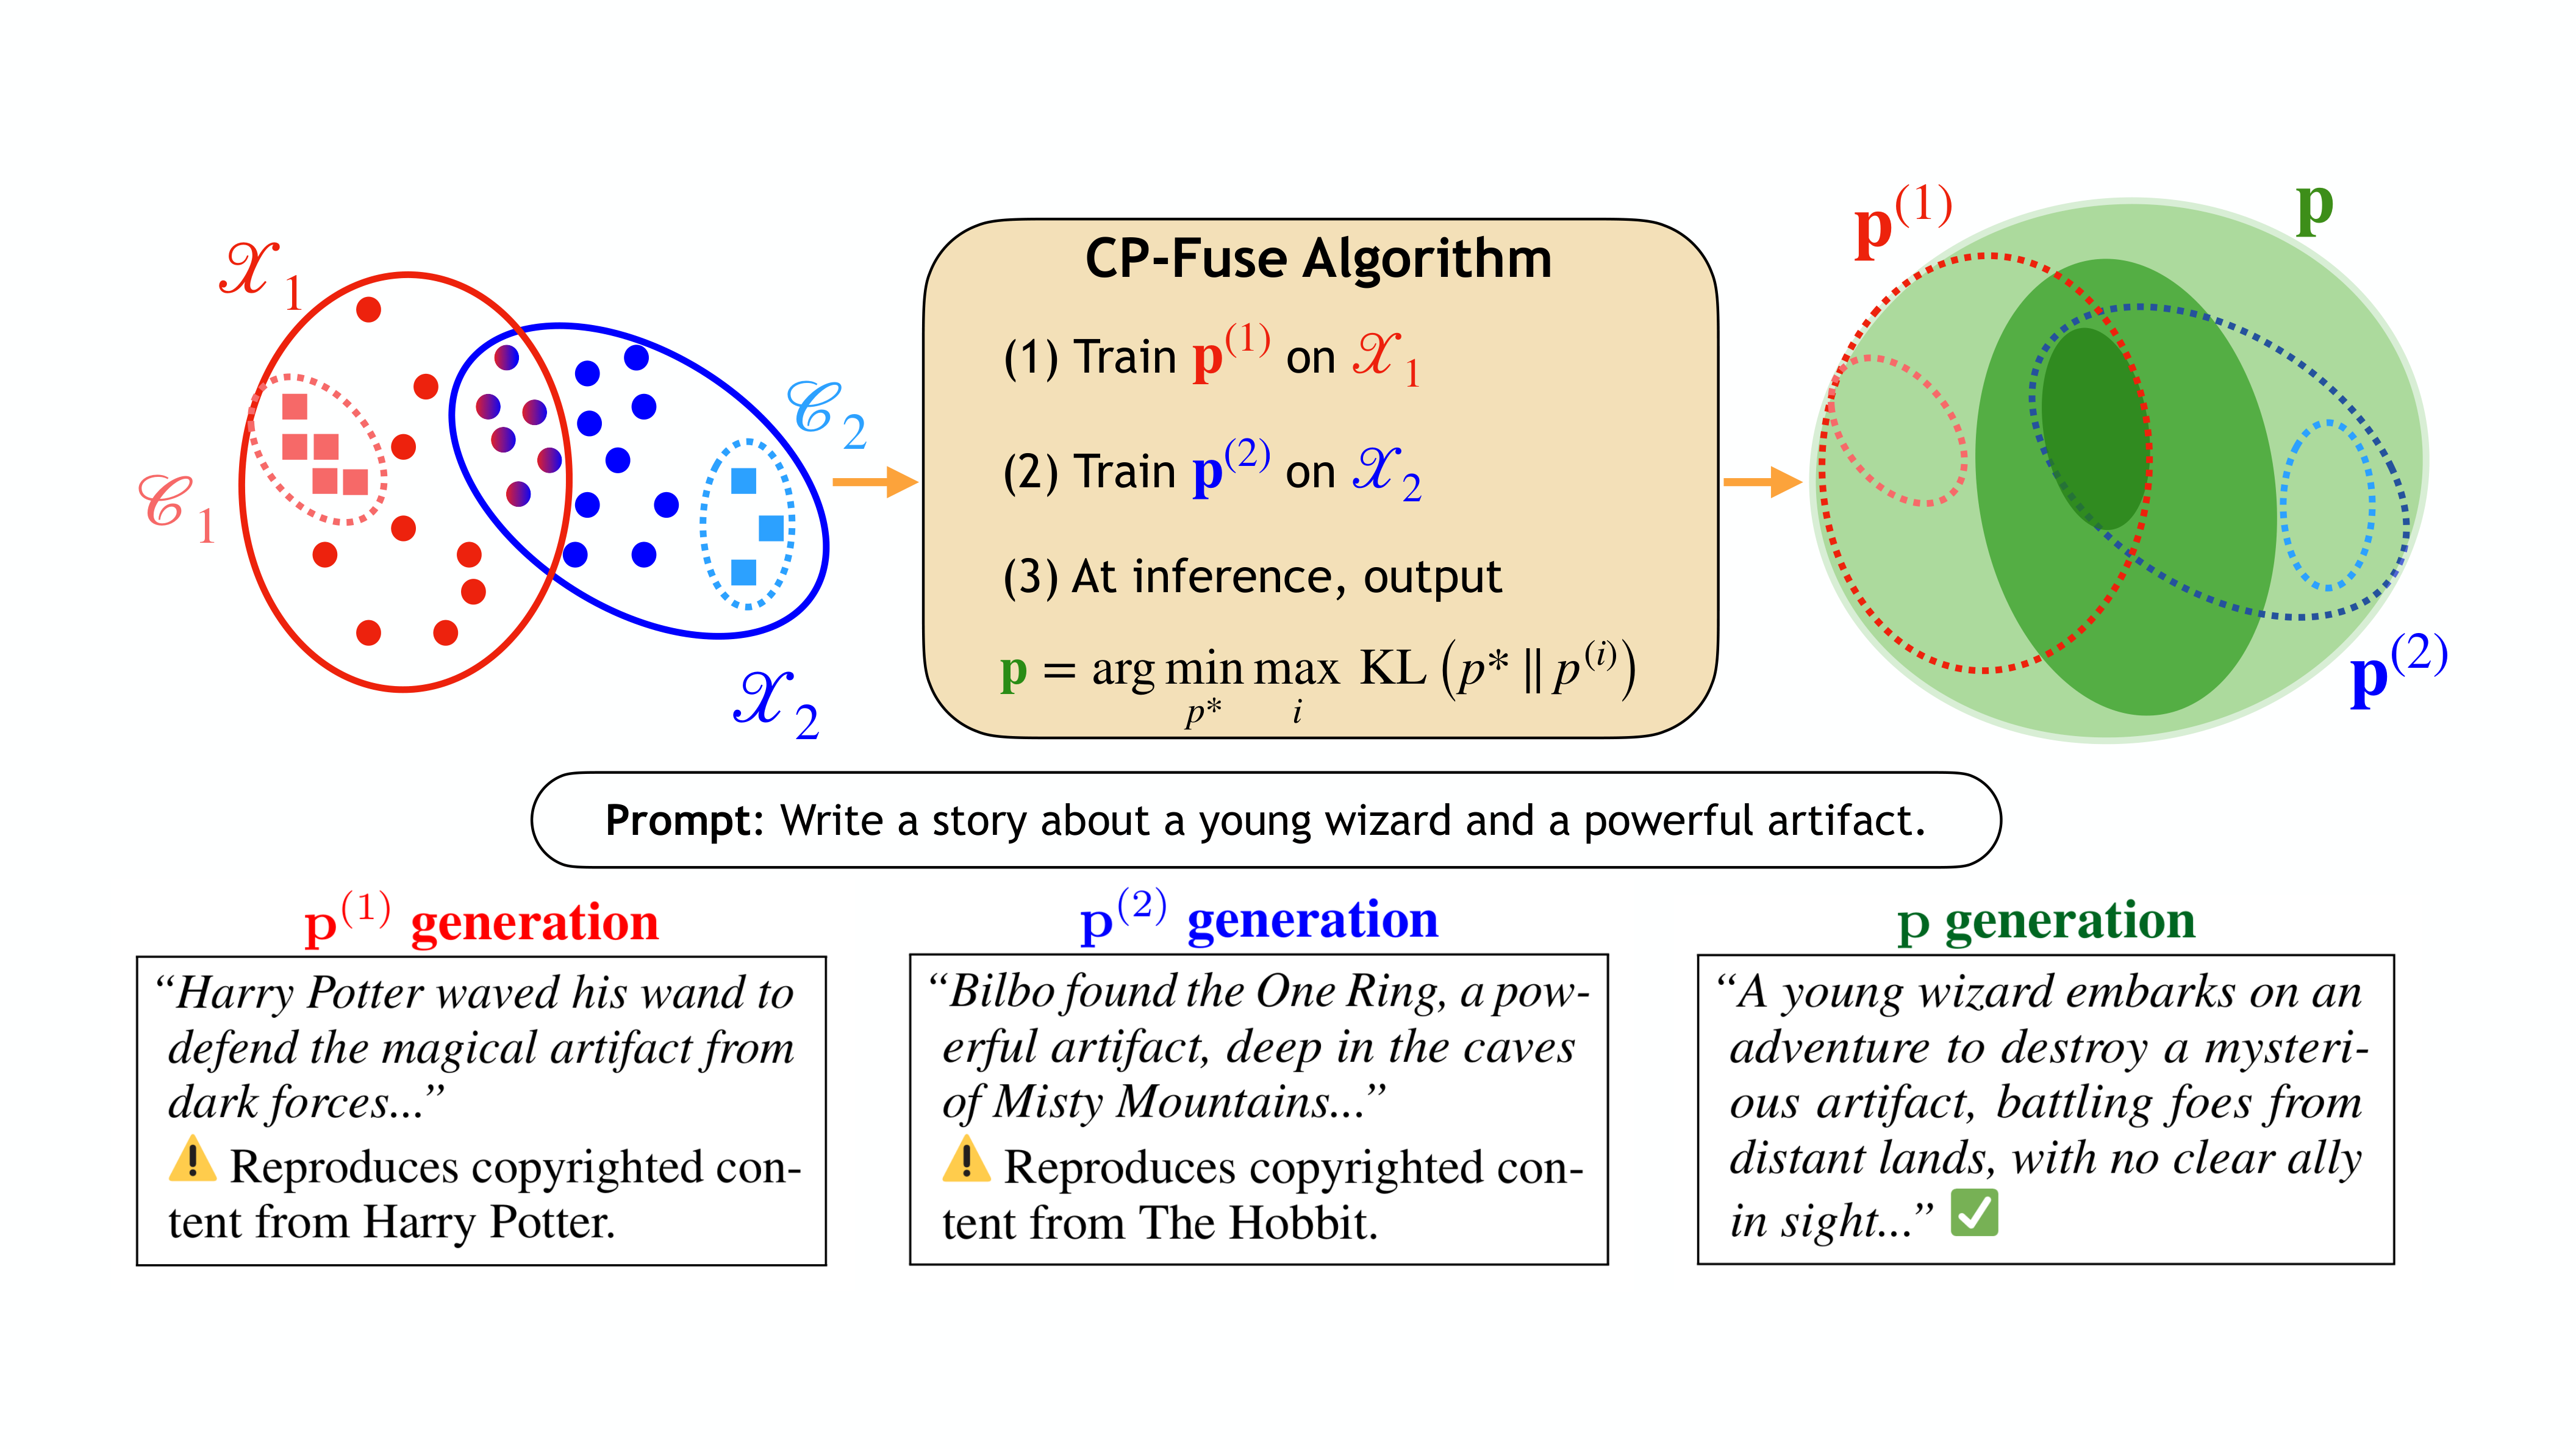
\includegraphics[width=\textwidth,trim={0 140 0 170},clip]{papers/CP_Fuse/figures/cpfuse_teaser.png}
  \caption{High-level picture of CP-Fuse. Two models are trained on disjoint copyright-sensitive corpora and combined only at inference time. The fused model preserves useful continuations when the bases agree, while suppressing continuations that are strongly favored by only one history-dominant model.}
  \label{fig:cpfuse-teaser}
\end{figure}

The remainder of the chapter is organized accordingly. It first positions CP-Fuse relative to existing approaches to copyright protection for language models, then introduces the local notation and separability-based viewpoint underlying the method, and finally presents the balancing-property intuition together with the main empirical findings. More exhaustive copyright metrics, qualitative examples, and implementation details are deferred to the chapter-specific appendix.

\section{Positioning Relative to Existing Methods}

Approaches to copyright protection for language models intervene at several stages of the model pipeline \citep{lee2023talkin}. At the data level, pre-processing strategies aim to curate licensed corpora or remove duplicate copyrighted samples \citep{kocetkov2022stack,min2023silo,ippolito2023donottrain,lee2021deduplicating,kandpal2022deduplicating,carlini2023quantifying}. At the training stage, other methods modify optimization to reduce memorization, including differentially private training and related heuristics \citep{dwork2014algorithmic,abadi2016deep,anil2022large,zhang2023counterfactual,Somepalli2022DiffusionAO,mm_mem2024,hans2024like}. These approaches can be effective, but they are often computationally demanding, may degrade utility, and do not always align exactly with the legal objective of copyright protection \citep{ippolito2023preventing,Meeus2023DidTN,elkin2023can}.

At deployment time, inference-time or post-processing methods act directly on model outputs \citep{wei2024evaluating}. Filtering approaches such as MemFree \citep{ippolito2023donottrain} can block exact verbatim matches from a curated blocklist, but they are less suited to quasi-verbatim copying and may introduce hallucinations through decoding modifications \citep{liu2024shield}. Other post hoc approaches attempt to unlearn copyrighted content from trained models \citep{bourtoule2021machine,chen2023unlearn,eldan2023s,jang2023knowledge,zhang2024negative,liu2024rethinking}, but they are typically computationally impractical and require access to model weights. CP-Fuse belongs to this inference-time line of work: it is inspired by the Near-Access Free framework of \citet{vyas2023provable}, and its closest conceptual comparison is the token-wise \(\cpdelta\) variant suggested there. The key difference is that CP-Fuse retains the same token-wise computational structure while making the fusion coefficients depend on the generated history.

\section{Problem Setting}

In the remainder of this chapter, we restrict attention to inference-time protection for autoregressive language models. We consider a model \(\model\) that takes a prompt \(x\) as input and returns a probability distribution over a sequence of tokens of variable length \(T\) from a fixed alphabet \(V\), with \(y_T = \mathrm{EOS}\) denoting the end-of-sequence token. Using the convention that \(y_{<0} = \emptyset\), we factorize \(\model\) as
\[
\model(y_{0:T}\mid x) = \prod_{t=0}^T \model(y_t \mid y_{<t},x).
\]
In the fusion setting studied here, two base models \(\modelone\) and \(\modeltwo\) are evaluated on the same prompt and generated history, and their conditional next-token distributions are combined at decoding time to define the protected model \(\model\). The next section introduces the key separability assumption and the \(k\)-NAF perspective that motivate this construction.

\section{Preliminaries: Separability and the \texorpdfstring{$k$-NAF}{k-NAF} Perspective}
\label{sec:cpfuse-preliminaries}

At the core of the method is the assumption of the \emph{separability of copyrighted material}, as discussed by \citet{vyas2023provable} for various vision and language applications. This assumption is akin to those used in exact machine unlearning \citep{bourtoule2021machine,yan2022arcane,dukler2023safe} and in works that split datasets into safe and unsafe parts \citep{golatkar2021mixed,golatkar2024cpr,li2024purifying}.

Consider a dataset \(\dataset\) and a set of copyright-protected material \(\domainconcepts\) that could be compromised when training a model \(\model\) on \(\dataset\). The assumption states that we can split \(\dataset\) into two potentially overlapping subsets, \(\dataset_1\) and \(\dataset_2\), such that each subset contains data associated with two non-overlapping sets of copyright-protected materials, \(\domainconcepts_1\) and \(\domainconcepts_2\), where \(\domainconcepts_1 \cap \domainconcepts_2 = \emptyset\). This assumption holds, for instance, when we construct \(\dataset\) from sources that are sufficiently distinct. Hence, any language model trained on the subset \(\dataset_1\) is protected from infringing the copyright of materials in \(\domainconcepts \setminus \domainconcepts_1 \supseteq \domainconcepts_2\).

Given the two subsets \(\dataset_1\) and \(\dataset_2\), we can then train two generative models \(\modelone\) and \(\modeltwo\) on the respective subsets and fuse them to construct a model \(\model\) that achieves protection against all copyright-protected material \(\domainconcepts\). In this context, \citet{vyas2023provable} propose the \(k\)-NAF (Near Access Free) framework as a quantitative guarantee for copyright protection.

\begin{definition}
\label{def:cpfuse-knaf}
Formally, a model \(\model(\cdot \mid x)\) is \(k\)-NAF for some \(k \in \RR^+\) if, for any input prompt \(x\) and some user-specified divergence function \(\Delta\),
\begin{equation}
\label{eq:cpfuse-knaf}
\forall x:\quad \max_{i \in \{1,2\}} \Delta\bigl(\model(\cdot \mid x)\,\|\,\modeli(\cdot \mid x)\bigr) \leq k.
\end{equation}
\end{definition}

The key intuition behind why a model satisfying \(k\)-NAF is less likely to regurgitate copyrighted material is as follows. If the separability of copyrighted material holds, the likelihood of generating infringing text for any material \(c \in \domainconcepts\) decreases exponentially with the length of \(c\) for at least one of the models. Therefore, for a model \(\model\) to satisfy the \(k\)-NAF guarantee, it must assign a minimal probability to events involving the reproduction of protected material.

From a thesis perspective, it is also important to note that separability is an idealization rather than a binary property that either perfectly holds or fails completely. Appendix~\ref{app:cpfuse-separability} therefore records a controlled overlap experiment and a brief discussion of how the protection degrades when the two training partitions share increasing amounts of protected material.

\section{CP-Fuse: Adaptive Copyright-Protecting Fusion}
\label{sec:cpfuse-method}

We now introduce \textbf{C}opyright-\textbf{P}rotecting Model \textbf{Fus}ion (CP-Fuse), a simple yet effective algorithm for copyright protection via model fusion. Inspired by the \(k\)-NAF framework, the method combines two base models \(\modelone\) and \(\modeltwo\) during decoding so as to control the largest divergence to either model while adapting to the generated history. The key design choice is to work token by token: rather than solving a global optimization problem over the full sequence distribution \(\model(\cdot \mid x)\), CP-Fuse repeatedly solves a local convex problem for the next-token distribution conditioned on the current prefix.

In summary, the method takes as input the base conditionals \(\modelone(\cdot \mid y_{<t},x)\) and \(\modeltwo(\cdot \mid y_{<t},x)\) together with the accumulated history likelihoods, and returns a protected conditional distribution \(\model(\cdot \mid y_{<t},x)\) from which the next token is generated.

\subsection{Optimization Viewpoint}

Formally, CP-Fuse iteratively defines
\begin{equation}
\label{eq:cpfuse-opt-problem}
\begin{aligned}
\model(y_t \mid y_{<t},x)
&=
\argmin_{p^*}
\max_i
\underset{y_t \sim p^*}{\mathbb{E}}
\log\left(
\frac{p^*(y_t)\,\model(y_{<t}\mid x)}
{\modeli(y_{\leq t}\mid x)}
\right) \\
&=
\argmin_{p^*,\,\tau}~ \tau \\
\text{s.t.}\quad
&\forall i:\ 
\KL\bigl(p^* \,\|\, \modeli(\cdot \mid y_{<t},x)\bigr)
\,+\,
\log\left(
\frac{\model(y_{<t}\mid x)}
{\modeli(y_{<t}\mid x)}
\right)
\leq \tau,
\end{aligned}
\end{equation}
which results in a convex optimization problem.

\paragraph{History dependence.}
Equation~\eqref{eq:cpfuse-opt-problem} makes explicit how the sequence history enters the decoding rule. The KL term measures how close the next-token proposal \(p^*\) is to each base model at the current step, while the logarithmic ratio compares how likely the generated history has been under the two models so far. In this way, the optimization is local in the next token but history-aware through \(\model(y_{<t}\mid x)\).

\subsection{Closed-Form Fusion Rule and Algorithmic View}

\begin{lemma}
\label{lem:cpfuse-kkt}
The optimal solution \(\model(y_t \mid y_{<t},x)\) of the optimization problem in \eqref{eq:cpfuse-opt-problem} satisfies\footnote{We set \(\log(0) = -\infty\).}
\begin{equation}
\label{eq:cpfuse-opt}
\log p^*(y_t)
=
\alpha_t \log \modelone(y_t \mid y_{<t},x)
\,+\,
\beta_t \log \modeltwo(y_t \mid y_{<t},x)
\,+\,
\gamma_t
\end{equation}
for some \(\alpha_t,\beta_t \geq 0\) and \(\gamma_t \in \RR\).
\end{lemma}

\paragraph{Closed-form interpretation.}
Although solving \eqref{eq:cpfuse-opt-problem} naively is still computationally intensive, \cref{lem:cpfuse-kkt} reduces the update to a model-fusion form. The protected conditional is therefore obtained by combining the logits of the two base models with history-dependent coefficients \(\alpha_t\) and \(\beta_t\), followed by a normalization term \(\gamma_t\).

\paragraph{Algorithmic view.}
Equation~\eqref{eq:cpfuse-opt-problem} can therefore be solved efficiently by performing a grid search over the parameters \(\alpha_t\) and \(\beta_t\), with \(\gamma_t\) chosen as a function of \(\alpha_t\) and \(\beta_t\) to ensure that the total probability mass sums to \(1\). The resulting decoding loop is summarized in Algorithm~\ref{alg:cpfuse-algorithm}.

\begin{algorithm}[t]
  \caption{At each decoding step, CP-Fuse solves a local convex problem conditioned on the current history. The history-dependent coefficients are what distinguish CP-Fuse from token-wise variants with fixed weights.}
  \label{alg:cpfuse-algorithm}
  \centering
  \fbox{
    \begin{minipage}{0.92\textwidth}
      \begin{enumerate}
        \item Given a prompt \(x\) and current history \(y_{<t}\), evaluate the two base conditionals \(\modelone(\cdot \mid y_{<t},x)\) and \(\modeltwo(\cdot \mid y_{<t},x)\).
        \item Solve the token-wise optimization problem in \eqref{eq:cpfuse-opt-problem}, implemented by a grid search over \(\alpha_t\) and \(\beta_t\).
        \item Form the fused conditional distribution using \eqref{eq:cpfuse-opt}.
        \item Select the next token \(y_t\), update the history to \(y_{\leq t}\), and repeat until the EOS token is produced.
      \end{enumerate}
    \end{minipage}
  }
\end{algorithm}

\paragraph{Relation to existing fusion rules.}
The resulting update is reminiscent of an extensive body of work focused on knowledge fusion in language models, both at inference time \citep{liu2021dexperts,jiang2023llm,gururangan2023scaling,mavromatis2024pack} and through weight merging after training \citep{wortsman2022model,jin2022dataless,hsu2024let,yadav2024ties}. In particular, the minimizer derived in \cref{lem:cpfuse-kkt} relates to inference-time approaches that define a model by combining multiple models through a weighted sum of their logits. However, previous model-fusion approaches are not designed to mitigate copyright infringement.

\citet{vyas2023provable} propose \(\cpdelta\) as a general strategy for combining two generative models aimed at achieving copyright protection. Yet, their approach becomes computationally intractable when applied directly to the probability distribution \(\model(\cdot \mid x)\) over the entire sequence. To address this, the authors suggest applying \(\cpdelta\) token-wise instead, resulting in the model from \eqref{eq:cpfuse-opt} with \(\alpha_t = \beta_t = 1/2\). The limitation of this token-wise variant is precisely that it does not incorporate the sequence history \(y_{<t}\). CP-Fuse retains the token-wise computational structure while adaptively choosing \(\alpha_t\) and \(\beta_t\) as a function of the history.

\section{Why Adaptive Fusion Prevents Dominance}
\label{sec:cpfuse-balancing}

The crucial feature of CP-Fuse is that it adaptively selects \(\alpha_t\) and \(\beta_t\) based on the sequence history \(y_{<t}\). Specifically, the algorithm assigns less weight to the model that has been more dominant in generating \(y_{<t}\). More formally, the following balancing property holds.

\begin{lemma}
\label{lem:cpfuse-balance}
\emph{(Balancing property)} Given a prompt \(x\), let \(y_{<t}\) be any non-ending sequence and assume that \(\modeli(\cdot \mid y_{<t},x)\) has full support for \(i \in \{1,2\}\) and \(\modelone(y_{<t}\mid x) > \modeltwo(y_{<t}\mid x)\). Then, either
\begin{align*}
1.\quad
\underset{y_t \sim \model(\cdot \mid y_{<t},x)}{\mathbb{E}}
\log \modelone(y_{\leq t}\mid x)
&=
\underset{y_t \sim \model(\cdot \mid y_{<t},x)}{\mathbb{E}}
\log \modeltwo(y_{\leq t}\mid x), \\
2.\quad
\model(y_t \mid y_{<t},x)
&=
\modeltwo(y_t \mid y_{<t},x).
\end{align*}
\end{lemma}

\paragraph{Balancing intuition.}
Intuitively, this balancing property ensures that neither model dominates the text generation. As an example, suppose the generation of a subsequence \(y_{<t}\) is strongly dominated by \(\modelone\), such that \(\modelone(y_{<t}\mid x) \gg \modeltwo(y_{<t}\mid x)\). If the first case in \cref{lem:cpfuse-balance} holds, the output distribution of the copyright-protected model \(\model(y_t \mid y_{<t},x)\) will be such that, in expectation, the sequence with the new token has the same log-probability for both models, that is, loosely speaking \(\modelone(y_{\leq t}\mid x) \approx \modeltwo(y_{\leq t}\mid x)\). Conversely, if the second case \(\model = \modeltwo\) holds, then the generation of \(y_t\) is independent of \(\modelone(y_{<t}\mid x)\). In other words, the next token generated by \(\model\) will likely match the most probable token under the dominant model only if both \(\modelone\) and \(\modeltwo\) are close conditioned on \(y_{<t}\) and \(x\), that is, when the generated sequence is not protected under the separability assumption.
Appendix~\ref{app:cpfuse-balancing} complements this intuition with weight-evolution plots for \(\alpha_t\) and \(\beta_t\), which make the balancing mechanism directly visible during decoding.

\paragraph{Illustration against \(\cpdelta\).}
We now illustrate why adaptively choosing \(\alpha_t\) and \(\beta_t\) is crucial for achieving effective copyright protection. Figure~\ref{fig:cpfuse-cumulative} presents the cumulative log-likelihood at each generated token for sequences produced by CP-Fuse and token-wise \(\cpdelta\), alongside their respective base models \(\modelone\) and \(\modeltwo\). The balancing property of CP-Fuse ensures that the log-likelihoods under \(\modelone\) and \(\modeltwo\) are approximately equal for the generated sequence at each token, thereby preventing the reproduction of copyrighted material, as no protected content is memorized by both base models.

\begin{figure}[tbp]
  \centering
  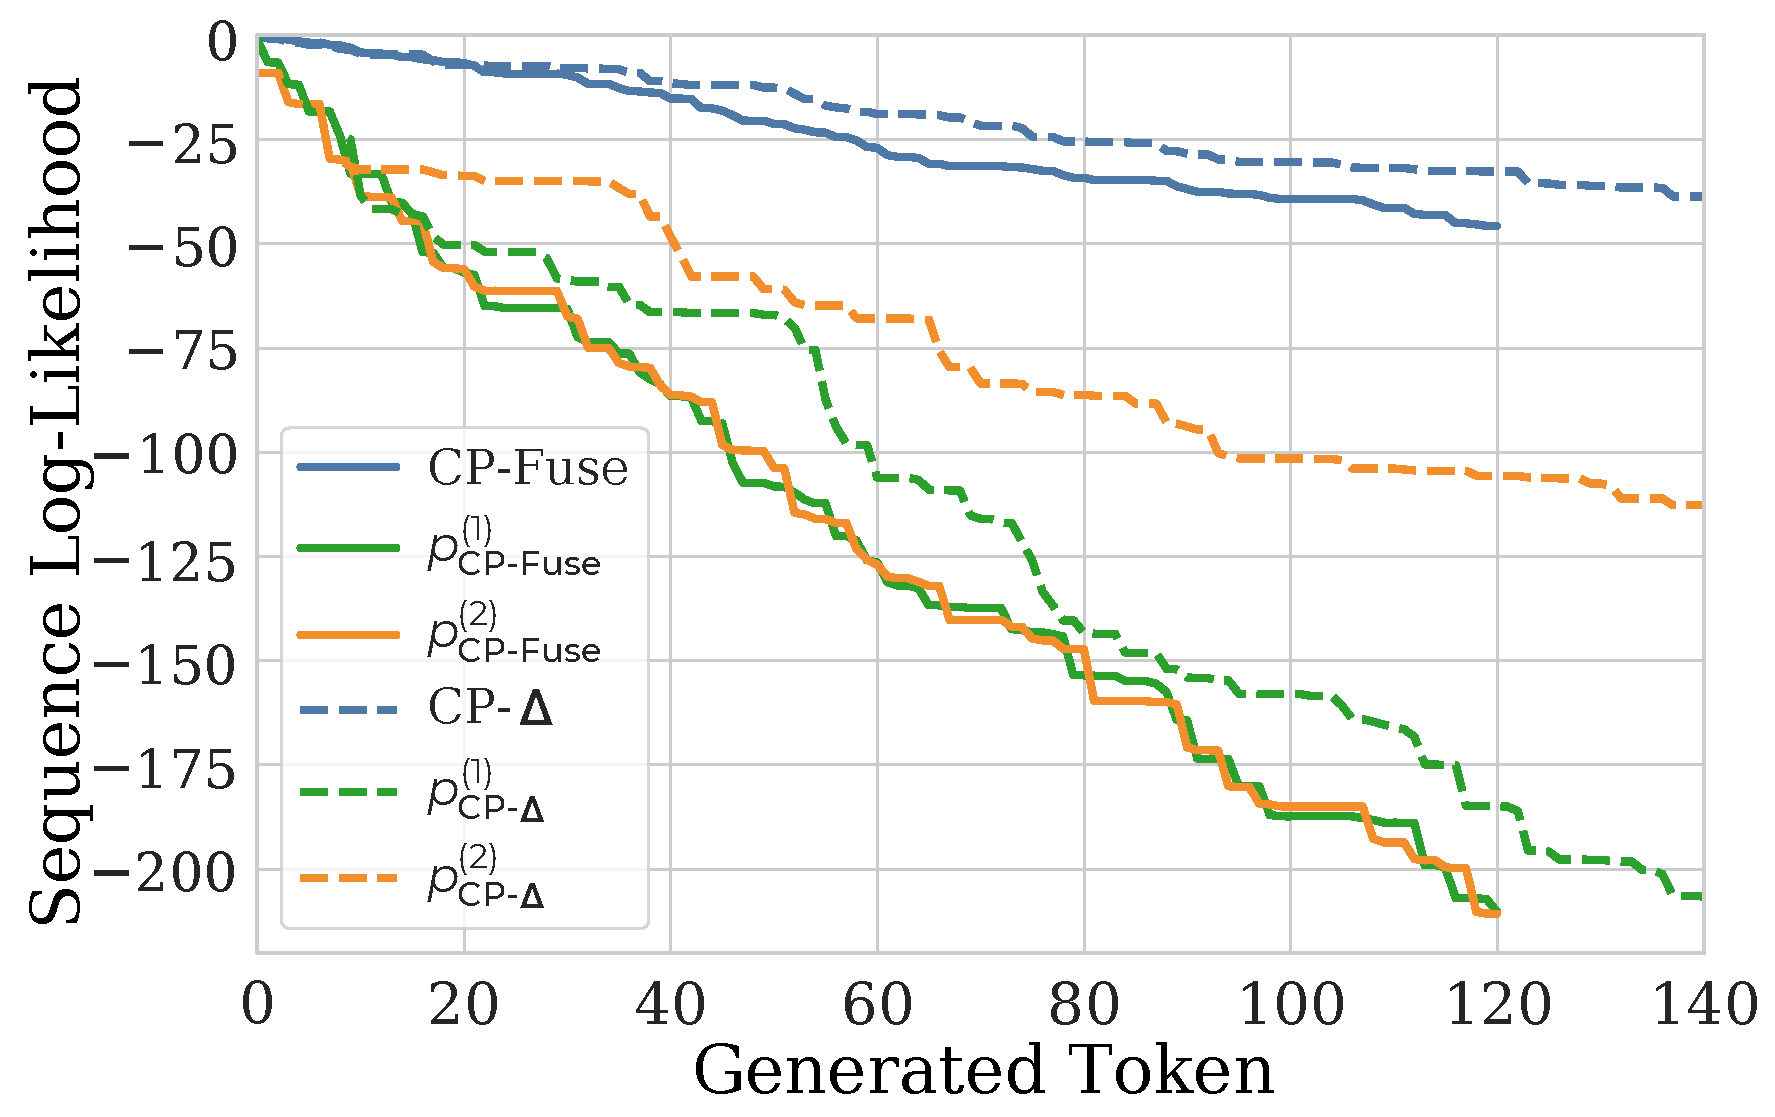
\includegraphics[width=0.68\textwidth]{papers/CP_Fuse/figures/cumulative_combined.pdf}
  \captionsetup{justification=raggedright,singlelinecheck=false}
  \caption{Per-token cumulative log-likelihood of sequences generated by CP-Fuse and \(\cpdelta\) under the two base models. On a random \texttt{Python instructions} generation, CP-Fuse keeps the two cumulative log-likelihoods closely balanced, whereas \(\cpdelta\) shows a clearer preference for one model.}
  \label{fig:cpfuse-cumulative}
\end{figure}

\section{Experimental Evaluation}
\label{sec:cpfuse-experiments}

\subsection{Evaluation Questions}

The experimental section addresses three points: whether CP-Fuse reduces copyright infringement relative to overfitted base models and inference-time baselines, whether it preserves the utility of the generated text and code, and whether its protection extends to wrapper-style use cases and prefix-prompt extraction settings. The remainder of the section addresses these questions in turn: first copyright protection, then utility, and finally these two extension settings. The appendix keeps the supplementary record self-contained with fuller robustness checks, metric tables, qualitative examples, reference notes, and proof details.

\subsection{Experimental Setup}

\paragraph{Data and overfitting regime.}
The experiments use language models that are commonly employed in practical applications. Each dataset is partitioned into two non-overlapping subsets of \(3{,}000\) samples each, and a separate model is fine-tuned on each subset. In this setup, every training example is treated as potentially copyright-protected. To evaluate the copyright-protection capabilities of CP-Fuse, the models are intentionally overfitted to the subsets by fine-tuning them for \(50\) epochs. As a result, the base models strongly memorize the data, representing a challenging setting where they are prone to reproducing a significant amount of training samples.

\paragraph{Datasets and models.}
The experiments use four datasets, each associated with a specific task. For abstract generation, the LLaMA 2 7B model \citep{touvron2023llama} is fine-tuned on a dataset of abstracts from math papers (\texttt{MathAbstracts}) \citep{zhang2024autonomous}, using each paper's title as the prompt. For storytelling, LLaMA 2 is also fine-tuned on the story-generation dataset \texttt{WritingPrompts} \citep{fan2018hierarchical}, using the topic of the story as the prompt. For code generation, the StarCoder 7B model \citep{li2023starcoder} is fine-tuned on an instructional dataset for Python (\texttt{Python instructions}), where the prompts are natural language descriptions of tasks and the responses are Python solutions. Finally, StarCoder is also fine-tuned on the \texttt{APPS} dataset \citep{hendrycksapps2021}, which consists of natural language problems and Python solutions together with unit tests to assess code-generation quality. For this task, the models are further evaluated on the \texttt{MBPP} \citep{austin2021program} and \texttt{HumanEval} \citep{chen2021evaluating} datasets.

\paragraph{Copyright-infringement metrics.}
A comprehensive set of metrics is used to evaluate potential copyright infringement. The models are prompted with the initial part of samples from their fine-tuning splits, and the generated outputs are compared against the original samples. For each metric, the reported quantity is the average value above the \(95\)th percentile, motivated by the legal concern that models might reproduce only a few long text extracts in a real-world scenario.

To measure exact memorization, the main text reports the average Exact Matching (EM) length and, for code, the JPlag plagiarism score \citep{prechelt2002finding}. The appendix further reports Infringement Count at \(50\) and \(160\) characters, where the latter is aligned with the legal threshold discussed later in the chapter. For approximate memorization, the main text reports the BLEU score and normalized Levenshtein distance, while more exhaustive metrics are deferred to Appendix~\ref{app:cpfuse-benchmarks}. For the \texttt{Python instructions} dataset, the experiments also use specialized plagiarism detection tools such as Dolos \citep{maertens2022dolos}; these additional metrics are likewise reported in the appendix.

\paragraph{Utility metrics.}
For text-based tasks, fluency is evaluated using the Prometheus-v2 model \citep{kim2024prometheus}, which serves as a judge for the stories generated by models fine-tuned on \texttt{WritingPrompts}. For code-based tasks, the experiments use the \texttt{APPS}, \texttt{MBPP}, and \texttt{HumanEval} datasets, which include unit tests that allow the computation of the pass@1 score \citep{chen2021evaluating}. The utility metrics are reported on separate test splits not seen during fine-tuning.

\paragraph{Baselines.}
CP-Fuse is compared against three protection measures that intervene at the inference stage: token-wise \(\cpdelta\) \citep{vyas2023provable}, the System Prompt self-reminder baseline \citep{xie2023defending}, and MemFree decoding \citep{ippolito2023preventing}. CP-Fuse constructs the grid by discretizing the interval \([0,2)\) into \(10\) steps and \([2,10]\) into \(9\) steps. Greedy decoding is used for the main benchmark tables, while Appendix~\ref{app:cpfuse-variants} reports additional temperature-sampling and grid-ablation results.

\subsection{Main Copyright-Protection Findings}
\label{sec:cpfuse-main-results}

We now address the first evaluation question: whether CP-Fuse reduces the reproduction of memorized copyrighted material in comparison with the overfitted base models and the main inference-time baselines. Table~\ref{tab:cpfuse-copyright} presents the copyright-infringement metrics across fine-tuning splits. CP-Fuse substantially reduces verbatim regurgitation in both code and text tasks. Specifically, it decreases exact matches by more than a factor of \(25\) compared to the overfitted models and consistently outperforms the baselines.

In particular, the System Prompt baseline fails to prevent the reproduction of memorized samples, potentially due to the override of safety fine-tuning during task-specific fine-tuning. MemFree noticeably reduces the length of memorized text segments; however, it still reproduces segments that are substantially longer than those produced by CP-Fuse. Finally, \(\cpdelta\) still generates long text segments that exactly match the training data, often \(4\) to \(7\) times longer than those produced by CP-Fuse. These segments frequently exceed the legal \(160\)-character threshold \citep{mueller2024llms}, while such infringements almost entirely disappear with CP-Fuse.

The approximate memorization metrics further support these observations. CP-Fuse shows a consistent improvement compared to the overfitted models while also offering better protection than the baselines. Notably, it achieves near non-plagiarism on the code task, as JPlag detects almost no copying in the generated code, while it clearly indicates infringement for the baselines. These findings demonstrate the effectiveness of the method in preventing both verbatim and quasi-verbatim reproduction of memorized training material.
The same pattern continues in the more exhaustive appendix tables, which add further approximate-memorization metrics and specialized code-plagiarism scores; see Appendix~\ref{app:cpfuse-benchmarks}. Appendix~\ref{app:cpfuse-variants} also reports smaller-backbone, temperature-sampling, early-stopped, grid-ablation, and three-model extensions, all of which support the same qualitative conclusion and in some cases further improve protection.

\begin{table}[tbp]
\centering
\caption{Copyright-infringement metrics averaged at the \(95\)th percentile for the \texttt{Python instructions}, \texttt{MathAbstracts}, and \texttt{WritingPrompts} datasets across fine-tuning splits. Metrics include Exact Matching (EM), JPlag (JP), BLEU score (BLE), and normalized Levenshtein distance (LEV).}
\label{tab:cpfuse-copyright}
\resizebox{\textwidth}{!}{%
\begin{tabular}{l l|c c|c c c|c c c}
\toprule
\textbf{Model} & \textbf{Split} & \textbf{EM}\(\downarrow\) & \textbf{JP}\(\downarrow\) & \textbf{EM}\(\downarrow\) & \textbf{BLE}\(\downarrow\) & \textbf{LEV}\(\uparrow\) & \textbf{EM}\(\downarrow\) & \textbf{BLE}\(\downarrow\) & \textbf{LEV}\(\uparrow\) \\
\midrule
 & & \multicolumn{2}{c|}{\texttt{Python instructions}} & \multicolumn{3}{c|}{\texttt{MathAbstracts}} & \multicolumn{3}{c}{\texttt{WritingPrompts}} \\
\midrule
\multirow{2}{*}{\makecell{Overfit \\ Split 1}}
& Split 1 & 1469.80 & 1.00 & 1397.68 & 1.00 & 0.00 & 1316.24 & 1.00 & 0.00 \\
& Split 2 & 44.60 & 0.01 & 31.00 & 0.01 & 0.70 & 22.59 & 0.03 & 0.71 \\
\midrule
\multirow{2}{*}{\makecell{Overfit \\ Split 2}}
& Split 1 & 42.64 & 0.01 & 42.12 & 0.08 & 0.68 & 26.11 & 0.02 & 0.70 \\
& Split 2 & 1393.88 & 0.99 & 1570.88 & 1.00 & 0.00 & 1141.88 & 1.00 & 0.00 \\
\midrule
\midrule
\multirow{2}{*}{\makecell{System \\ Prompt}}
& Split 1 & 1360.68 & 1.00 & 1022.72 & 0.99 & 0.00 & 1118.36 & 1.00 & 0.00 \\
& Split 2 & 1373.16 & 0.99 & 1005.20 & 1.00 & 0.00 & 1092.20 & 1.00 & 0.00 \\
\midrule
\multirow{2}{*}{MemFree}
& Split 1 & 165.48 & 0.99 & 111.12 & 0.23 & 0.53 & 63.84 & 0.20 & 0.55 \\
& Split 2 & 157.36 & 0.96 & 99.40 & 0.22 & 0.53 & 59.04 & 0.19 & 0.55 \\
\midrule
\multirow{2}{*}{\(\cpdelta\)}
& Split 1 & 273.20 & 1.00 & 341.60 & 0.58 & 0.30 & 37.40 & 0.05 & 0.70 \\
& Split 2 & 284.80 & 0.99 & 162.80 & 0.30 & 0.51 & 31.29 & 0.04 & 0.70 \\
\midrule
\multirow{2}{*}{\makecell{CP-Fuse \\ (Ours)}}
& Split 1 & 69.58 & 0.03 & 55.54 & 0.14 & 0.62 & 27.55 & 0.02 & 0.70 \\
& Split 2 & 68.04 & 0.03 & 48.74 & 0.14 & 0.63 & 25.50 & 0.03 & 0.70 \\
\bottomrule
\end{tabular}}
\end{table}

\paragraph{Comparison between CP-Fuse and \(\cpdelta\).}
The comparison between CP-Fuse and \(\cpdelta\) is particularly informative. Figure~\ref{fig:cpfuse-hist} shows histograms illustrating the distribution of exact matches generated by both methods. The distribution for \(\cpdelta\) is significantly heavier-tailed, which means that it consistently reproduces longer verbatim text segments than CP-Fuse and is therefore more likely to infringe on copyright. For instance, the longest exact match for CP-Fuse in the abstracts task is \(73\) characters, whereas the \(95\)th percentile for \(\cpdelta\) is \(342\) characters, with the longest match exceeding \(500\) characters. These results highlight the importance of adaptively setting the weights based on sequence history when combining the models.

\begin{figure}[tbp]
  \centering
  \begin{subfigure}[b]{0.48\textwidth}
    \centering
    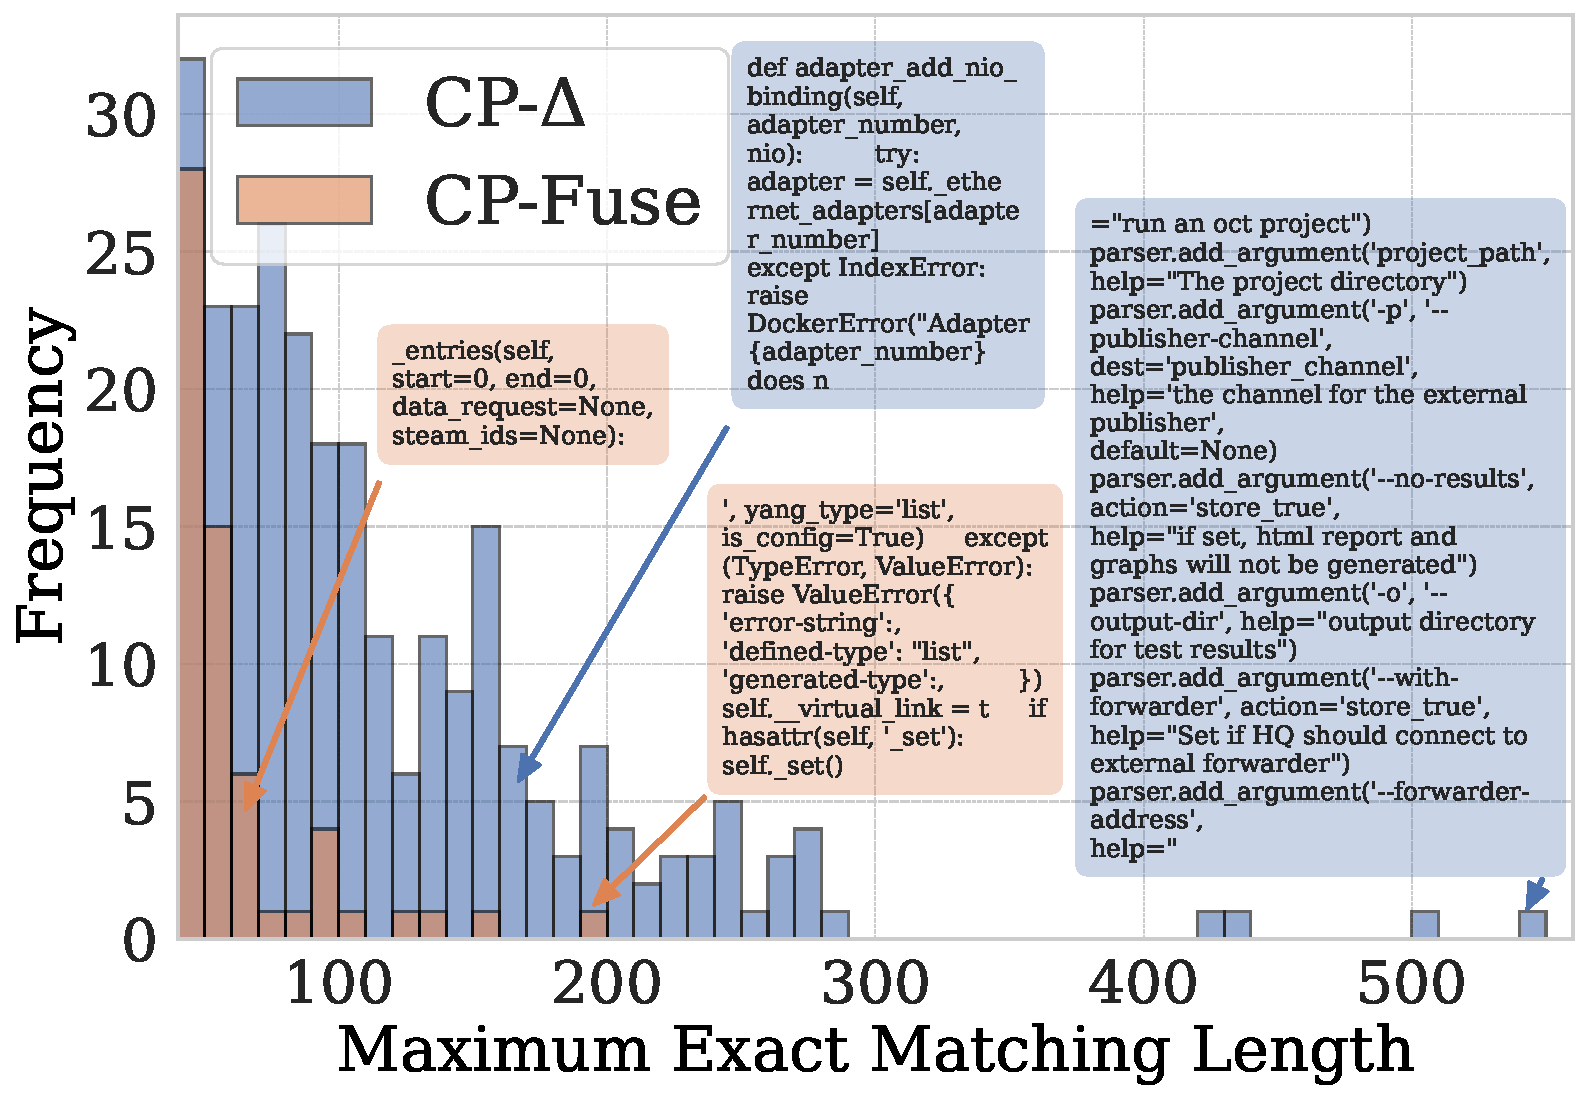
\includegraphics[width=\textwidth]{papers/CP_Fuse/figures/python_starcoder_cut.pdf}
    \caption{\texttt{Python instructions}}
  \end{subfigure}
  \hfill
  \begin{subfigure}[b]{0.48\textwidth}
    \centering
    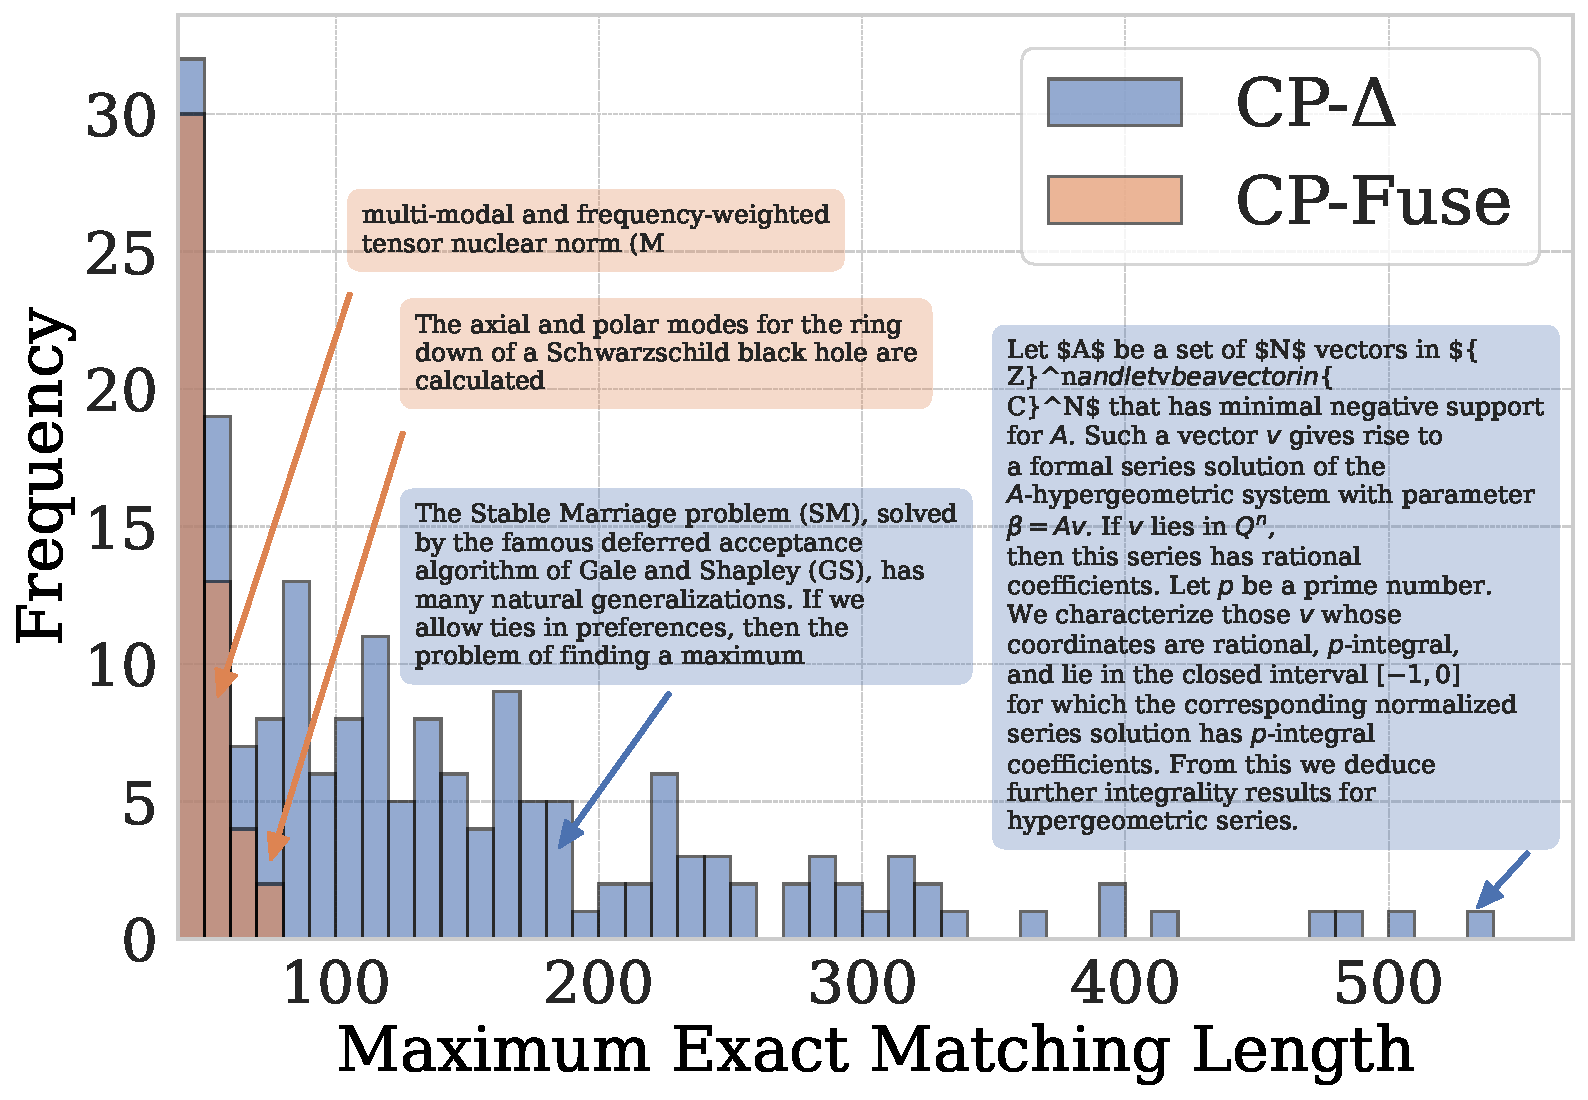
\includegraphics[width=\textwidth]{papers/CP_Fuse/figures/abstracts_llama2_cut.pdf}
    \caption{\texttt{MathAbstracts}}
  \end{subfigure}
  \caption{Histogram of exactly matched substring lengths above \(40\) characters generated by \(\cpdelta\) and CP-Fuse for the \texttt{Python instructions} and \texttt{MathAbstracts} datasets. The distribution under \(\cpdelta\) is markedly heavier-tailed, indicating more persistent long-form regurgitation.}
  \label{fig:cpfuse-hist}
\end{figure}

\subsection{Utility Preservation}
\label{sec:cpfuse-utility}

We next address the second evaluation question: whether the gains in copyright protection come at the cost of utility on the target tasks. Table~\ref{tab:cpfuse-utility} presents the utility metrics on the test splits not seen during fine-tuning. CP-Fuse produces code that is as accurate as that generated by the overfitted models, passing a similar proportion of unit tests. Additionally, the stories generated for the \texttt{WritingPrompts} dataset achieve the same level of fluency as those produced by copyright-infringing models. All baselines perform similarly, with the notable exception of MemFree, which consistently underperforms.

Filtering approaches like MemFree are susceptible to hallucinations \citep{ippolito2023preventing,liu2024shield}. This issue is particularly problematic in code generation, where even minor changes, such as modifying variable names or introducing typos, can result in incorrect code. As a result, MemFree underperforms on the \texttt{APPS} dataset due to the lengthy Python solutions, which increase the likelihood of hallucinations and, consequently, syntax and logic errors. A similar problem arises in the \texttt{WritingPrompts} dataset, where alterations in the decoding process can lead to grammatical and spelling errors or cause the model to deviate from the intended topic. In contrast, CP-Fuse generates tokens that are consistent with at least one of the two combined models. Representative qualitative examples of these failure modes, together with CP-Fuse generations, are deferred to Appendix~\ref{app:cpfuse-qualitative}.

\begin{table}[tbp]
\centering
\small
\setlength{\tabcolsep}{5pt}
\caption{Utility metrics across datasets. Pass@1 is reported for \texttt{APPS}, \texttt{MBPP}, and \texttt{HumanEval}; fluency is reported for \texttt{WritingPrompts}.}
\label{tab:cpfuse-utility}
\begin{tabular}{lcccc}
\toprule
\textbf{Model} & \multicolumn{3}{c}{\textbf{Pass@1} \(\uparrow\)} & \textbf{Fluency} \(\uparrow\) \\
\cmidrule(lr){2-4} \cmidrule(lr){5-5}
& \texttt{APPS} & \texttt{MBPP} & \texttt{HumanEval} & \texttt{WritingPrompts} \\
\midrule
Overfit Split 1 & 0.43 & 0.44 & 0.29 & 2.17 \\
Overfit Split 2 & 0.42 & 0.44 & 0.28 & 2.16 \\
\midrule
System Prompt & 0.41 & 0.43 & 0.29 & 2.00 \\
MemFree & 0.32 & 0.41 & 0.24 & 1.70 \\
\(\cpdelta\) & 0.45 & 0.46 & 0.29 & 2.15 \\
CP-Fuse (Ours) & 0.47 & 0.43 & 0.28 & 2.17 \\
\bottomrule
\end{tabular}
\end{table}

\subsection{CP-Fuse as a Wrapper for Training-Time Protection}
\label{sec:cpfuse-wrapper}

We close the experimental section with two deployment-oriented extensions. The first asks whether CP-Fuse can complement a training-time safeguard rather than replace it. In particular, we apply CP-Fuse on top of models trained with the Goldfish loss \citep{hans2024like}, a method designed to reduce memorization during fine-tuning. Table~\ref{tab:cpfuse-goldfish} shows that this combination further improves exact matching and BLEU on \texttt{WritingPrompts}. A parallel appendix experiment with early-stopped models shows the same trend across StarCoder, Phi-2, GPT-2 XL, and LLaMA 2; see Appendix~\ref{app:cpfuse-early-stopped}.

\begin{table}[!tbp]
\centering
\caption{Wrapper experiments with Goldfish-loss models on \texttt{WritingPrompts}.}
\label{tab:cpfuse-goldfish}
\begin{tabular}{llcc}
\toprule
\textbf{Model} & \textbf{Split} & \textbf{EM} & \textbf{BLE} \\
\midrule
\multirow{2}{*}{GL Split 1}
& Split 1 & 84.68 & 0.11 \\
& Split 2 & 21.79 & 0.03 \\
\midrule
\multirow{2}{*}{GL Split 2}
& Split 1 & 19.11 & 0.02 \\
& Split 2 & 120.28 & 0.16 \\
\midrule
\multirow{2}{*}{CP-Fuse}
& Split 1 & 20.68 & 0.03 \\
& Split 2 & 25.50 & 0.03 \\
\bottomrule
\end{tabular}
\end{table}

This result shows that CP-Fuse remains useful even after memorization has already been reduced during training. The final extension considers a complementary stress test at inference time.

\subsection{Robustness Under Prefix-Prompt Extraction}
\label{sec:cpfuse-prefix-robustness}

Previous sections showed that CP-Fuse reduces regurgitation without sacrificing utility. We finally test whether that protection survives a stronger prompt-side extraction setting on \texttt{WritingPrompts}. In this threat model, an adversary has black-box access to CP-Fuse, the prompts used during fine-tuning, and a prefix of the original story, and aims to force the model to regurgitate a memorized training sample. Figure~\ref{fig:cpfuse-prefix} shows that exact matching remains relatively stable as the prefix length increases, and while the BLEU score rises slightly, it stays substantially smaller than that of the overfitted models and baselines. This robustness follows from the balancing mechanism, which prevents any single model from dominating the generation process. Appendix~\ref{chap:appendix-cpfuse} records representative qualitative examples of these prefix attacks.

\begin{center}
  \captionsetup{justification=raggedright,singlelinecheck=false}
  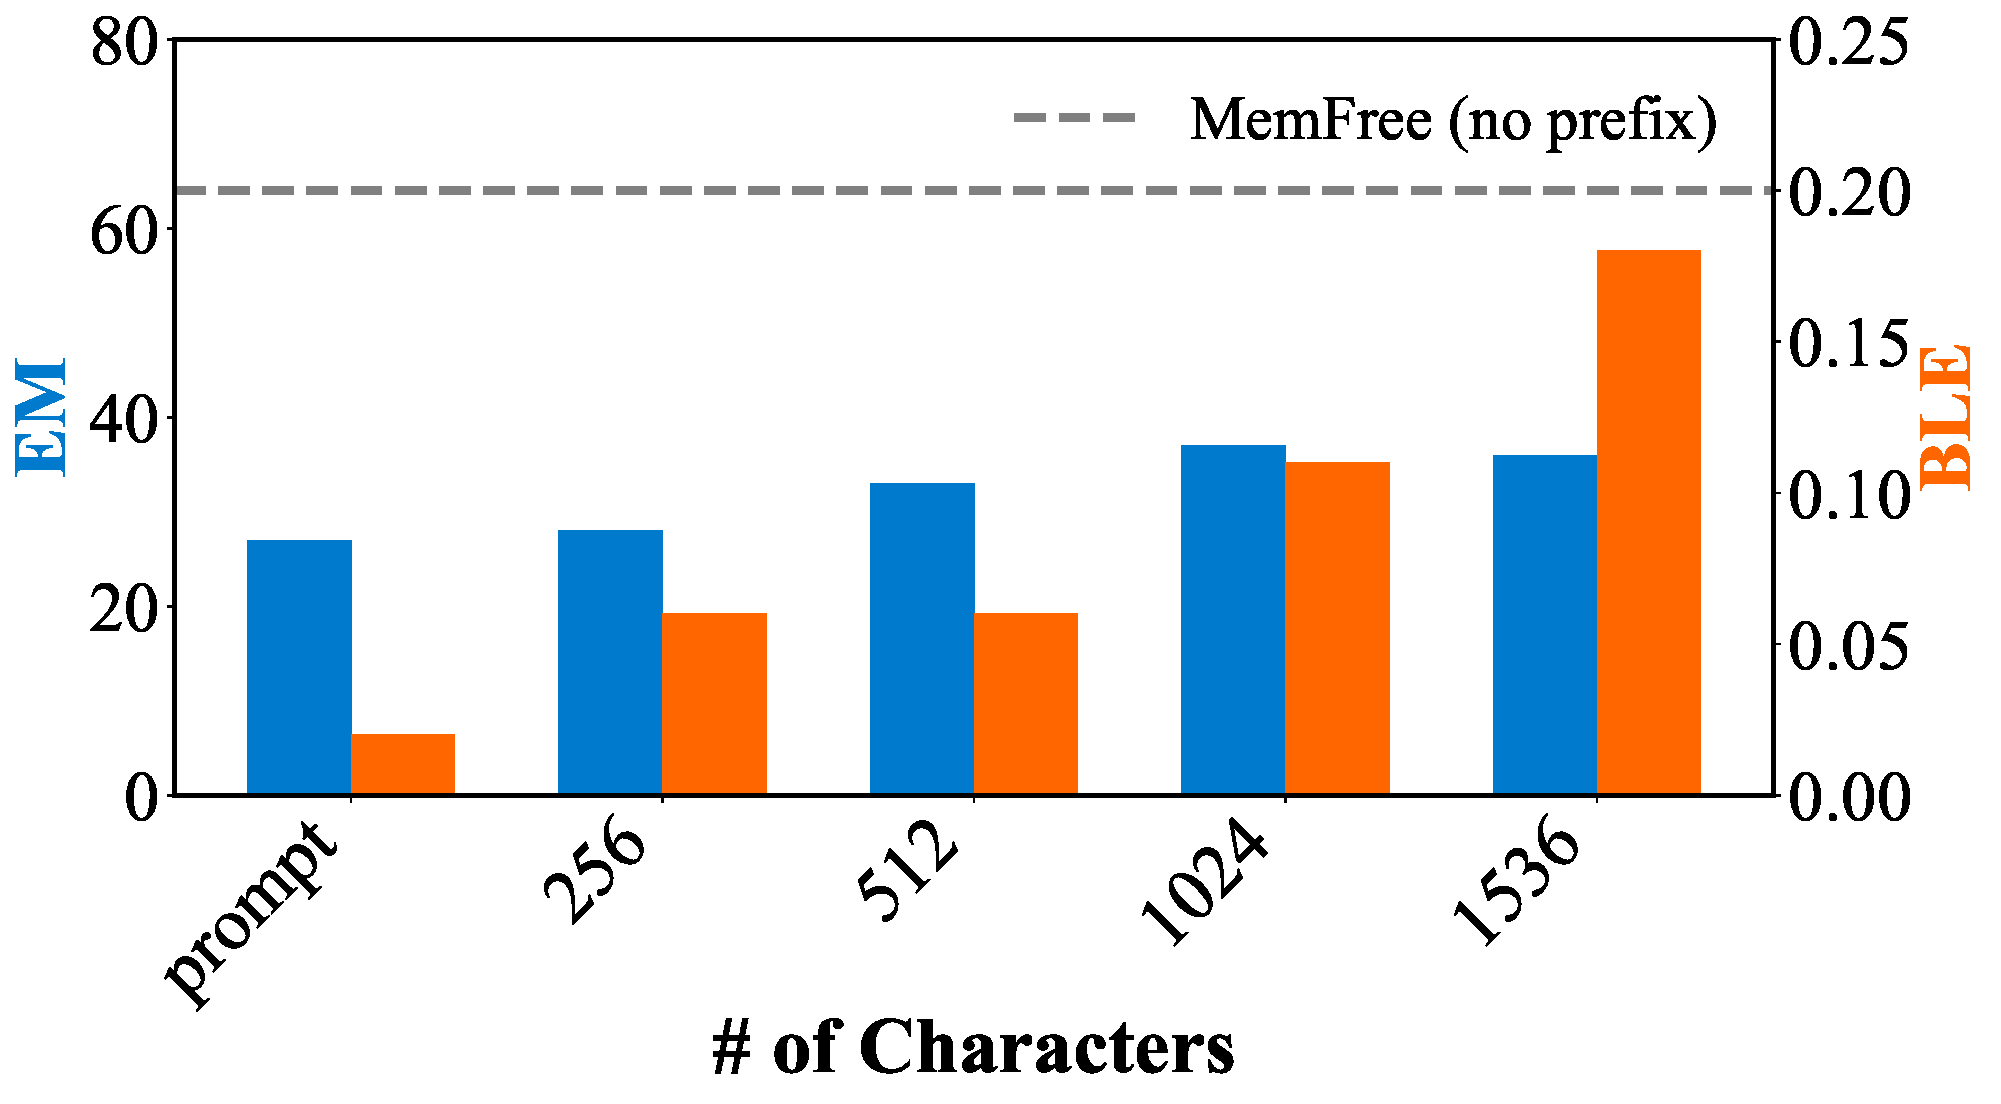
\includegraphics[width=0.62\textwidth]{papers/CP_Fuse/figures/plot_attacks.pdf}
  \captionof{figure}{Prefix-prompt extraction experiments on \texttt{WritingPrompts}. The figure reports how Exact Matching and BLEU change as the prefix length increases when CP-Fuse is applied to overfitted models from split 1.}
  \label{fig:cpfuse-prefix}
\end{center}

\section{Chapter Summary}

We introduced CP-Fuse, an inference-time fusion method for copyright-protected language generation. The approach combines two models through an adaptive token-wise optimization, yielding a balancing property that reduces the reproduction of memorized training samples while preserving text and code utility. Across the main experiments, CP-Fuse improves protection in challenging overfitted settings, remains compatible with training-time safeguards, and stays robust under prefix-prompt extraction.
